%************************************************
\chapter{Conclusions and Future Work}\label{ch:conclusions}
%************************************************

To finish this document, we sum up some conclusions from the work done, and results 
obtained. We will also enumerate some future lines of research.

\section{Conclusions}


In the memory of this project we try to show the work done from the beginning, but we only showed our right decisions, and the information that is significant for the final result. The truth is that, aside from the information included in this paper, we have worked with other systems that ended up discarded. This isn't a negative aspect, because if we didn't, for example, study the Contiki OS, Cooja simulator and the hardware used, we could not be sure the development of the first PoC for that system would be impossible in the time given.


With regard to the work presented, the flexibility of the computation offloading technique, identifying the key operations that can be delegated, and those ones that can't, has allowed us to define a general solution for the vast world of the Internet of Things. The IoT devices can operate as individual actors in the P2ABCE ecosystem, and when in need of performing computation offloading, the delegation server can also be a device considered into the IoT class.


% Resultados son válidos: feseability, problema de tiempo en sistemas de tiempo real
% Se han conseguido objetivos planteados
% Experiencia: qué era más tedioso, dificultades durante diseño y desarrollo
% Primera aproximación de este tipo ~~: más bien somos el future work de...
% Aplicación de procedimientos aprendidos/aplicados durante el TFG/carrera
% ^ Novelty


During the development, we had to investigate a lot of concepts related to IoT, smart cards, and even the insides of P2ABCE's code, to fix many existing bugs in the original project and minimize the amount of changes it had to undergo, in order to work with the IoT devices. In the implementation chapter we give guidelines to port MULTOS applications, considering the particularities we encountered, that's why we can't consider it an \textit{instruction manual to port MULTOS apps}, but an interesting reading on how to confront a similar project. For example, if we wanted the Idemix implementation from \citep{vullers2013efficient}, previous to P2ABCE, in a IoT device, we could apply almost the same steps, obtaining a core functionality of Idemix for constrained devices in C.

Our PoC implementation demonstrates that this project is actually feasible, not by performing a simulation of an IoT device, like in \citep{vanet}. However, the use of third party libraries and no hardware acceleration support, makes the PoC too slow for certain cases, e.g., a Real-Time system requires almost immediate operations, like a car warning that another one is approaching too fast.
There is a long path of research before we can see this design in production, as many decisions depend on the specific deployment in consideration.


Recalling the objectives listed in \autoref{objectives:section}, we think we accomplish them, except the implementation of a PoC in the most constrained device possible, where we used LEDE to ease our development, and the last objective, where we could have given a use to the PoC, and we leave as part of the future work. In spite of this negative auto-critic, we have to acknowledge that this is the first privacy-preserving ABC implementation for IoT, designed for extensibility, interoperability and maintenance.

Finally, we are very thankful to IBM's grant for the \textit{Privacy Preserving Identity Management applied to IoT} project, which allowed us to get this far. Also, in \autoref{ch:JCR} we show the version for publication in a JCR magazine.


\section{Future work}


Due to the nature of the project, there exist many options to continue researching in this area. We list below a collection of the tasks we couldn't accomplish but would have been our next steps:

\begin{itemize}
	\item Second PoC for Arduino systems
	
	We have already developed a working PoC for Linux based systems, and from our objective of using the most constrained devices available, we can follow an iterative process, building for devices a little more constrained than the last one. The next natural step, after building with LEDE/OpenWrt, is to aim for Arduino.
	
	The critical changes to the actual PoC are: 
	\subitem The transmission channel, if the device has no TCP/IP stack, it could use a Serial connection to transmit BIOSC and delegation messages.
	\subitem The use of a Json file to store the smart card status depends on whether the device has enough space or a file system. The current Json parser also uses too much dynamic memory. At this stage the serialization should be performed in a binary format, in a file or writing variables directly to the EEPROM memory.
	\subitem GMPLib and OpenSSL libraries must be replaced by others with similar capabilities, or special implementations for the particular device in use.
	
	All these changes affect only the \textit{external utilities} and \textit{interfaces} sections of the code, leaving the \textit{core} untouched, because the smart card logic doesn't change.
	
	\item Implement more P2ABCE functionality in the device
	
	If instead of aiming for more constrained devices, we work with similar devices to the Omega2, the computational power of the device could assume all the functionality of P2ABCE, at least for some roles. In a M2M (machine to machine) environment, the devices could act as Provers and Verifiers in the same interaction, and the verifying logic could be implemented entirely in the device (generate a Presentation Policy and checking a prove in a Presentation Token is valid), reducing the need of a delegation server.
	
	\item Improve the \textit{core smart card} code
	
	From the simple refactoring of removing the MULTOS reimplemented API for direct calls to the \textit{interfaces}, to identify all the \texttt{memcpy} copies of multiple variables with one call, removing the compiler directive for not using memory padding in the defined structures, letting the compiler manage the memory automatically.
	
	
	\item Use cryptographic hardware
	
	Atmel offers many solutions for secure memory and cryptographic operations chips, with serial interfaces for the IoT devices. We could benefit from this chips by storing the secret keys of the credentials inside the secure memory, and speed up the SHA256 and AES128 calculations, currently software implemented and slow compared to any hardware implementation. 
	
	
	
	\item Support Extended APDUs
	
	Currently, the APDU instruction handlers use the GET RESPONSE command to send large APDU Response Payloads, but we can reduce the number of APDUs exchanged supporting the Extended APDU format. Because the P2ABCE already sent some Extended APDUs, the APDU I/O interface in the PoC has support for Extended APDU Commands, but not for Extended Responses.
	
	\item Integrate the IoT+Idemix solution in FIWARE
	
	Our sixth objective, that we couldn't get to design in depth. The original idea was to integrate in a FIWARE\footnote{FIWARE \url{https://www.fiware.org/}} environment the Fiware Keyrock and Idemix Issuer, so both, users and IoT devices' identities are managed in the IdM\footnote{Identity Management - KeyRock \url{https://catalogue.fiware.org/enablers/identity-management-keyrock}} system. The Issuer generates credentials based on the user’s attributes held in the Keyrock, and IoT devices can authenticate against Fi-ware services (using Idemix), or authenticate against other IoT devices (M2M).
	
	\begin{figure}[bth]
		\begin{center}
			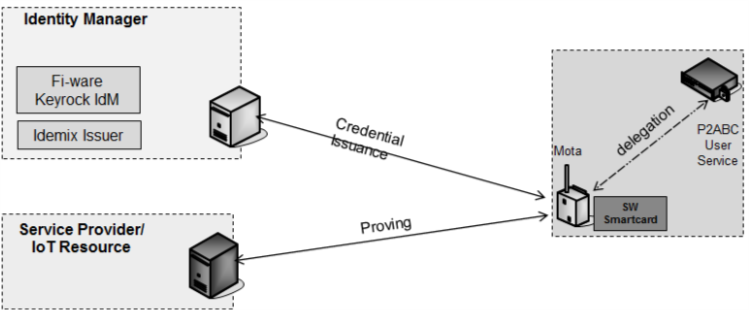
\includegraphics[width=0.8\linewidth]{gfx/fiware}
		\end{center}
		\caption{IoT+Idemix Fi-Ware integration.}
		\label{fig:fiware}
	\end{figure}

	\item Research P2ABCE policies for IoT applications
	
	The next step, after integrating Idemix with an Identity Management system, should be to design more complex applications to IoT scenarios. We talked about a smart building in the introduction, but the straightforward proofs we can present depend on the signed values in the credentials. The Zero-Knowledge Proofs cryptography is already implemented, we only have to extend the protocols to benefit from them.
	
	For example, a combination of authentication and arbitrary proof could be achieved by a combined proof of knowledge of a signed credential (current authentication system) and said arbitrary proof, although the values used in it aren't actually signed by the Issuer, the first proof gives credibility.
	
	Another solution for the same problem, similar to a PKI scheme, the IoT device receives a signed credential including an attribute which is his own public key. The IoT device can issue new credentials with the parameters it needs for the arbitrary proofs. The Verifier then certifies the new credential is signed by the IoT device's public key.
	
\end{itemize}


